در این فصل به بررسی اجمالی برخی از پژوهش‌ها و کارهای مرتبط با موضوع این پژوهش خواهیم پرداخت. در مورد هر یک از این موارد به ارتباط آن با بحث جاری، کاربرد و یا نقاط تأثیرگذار آن در موضوع این پژوهش و هم‌چنین ضعف ها و نقایص آن‌ها پرداخته شده است. 
\section{الگوهای برنامه‌نویسی همروند}
\label{section:actorPatterns}
در برنامه‌نویسی همروند با اکتور‌ها دو نوع الگوی کلی معرفی شده است \cite{Agha1990}: یکی  \textit{\gls{تقسیم-و-حل}}\LTRfootnote{devide and conquer} (برای این الگو از نام انشعاب و الحاق\LTRfootnote{fork and join} هم  یاد می‌شود) و دیگری \textit{\gls{خط لوله}}\LTRfootnote{pipeline}. 
در روش تقسیم-و-حل مسئله‌ی مورد بحث به زیربخش‌های کوچکتر و مستقل تقسیم می‌شود که هرکدام به صورت مستقل حل می‌شوند و نتایج هر زیربخش برای نتیجه‌گیری کلی ادغام می‌شوند. در برنامه‌نویسی به مدل اکتور، برای پیاده‌سازی این الگو یک اکتور رئیس\LTRfootnote{master} در نظر گرفته می‌شود که تعدادی اکتور کارگر\LTRfootnote{worker} را برای حل زیربخش‌های مسئله ایجاد می‌کند. عمل تقسیم به وسیله‌ی فرستادن پیغام‌ حاوی حالت لازم برای حل زیر بخش به کارگر‌ها انجام می‌شود. کارگرها به نوبه‌ی خود منطق لازم برای حل زیر بخش را ایجاد نموده و نتیجه را به صورت پیغام دیگری برای اکتور رئیس ارسال می‌کنند. نهایتا رئیس با ادغام نتایج جواب نهایی 
مسئله را تولید می‌کند. شایان ذکر است که فازهای تقسیم و حل لزوما توسط اکتور یکسان اجرا نمی‌شوند. ممکن است اجرای فاز حل به اکتور دیگری سپرده شود.\cite{Feng08scalablemodels}
مثال دیگری از پیاده‌سازی الگوی تقسیم-و-حل در مدل اکتور  در \cite{Feng08scalablemodels} آمده است که در آن الگوریتم جستجوی سریع\LTRfootnote{quick sort} توسط این الگو پیاده شده است.
\begin{figure*}
    \begin{center}
	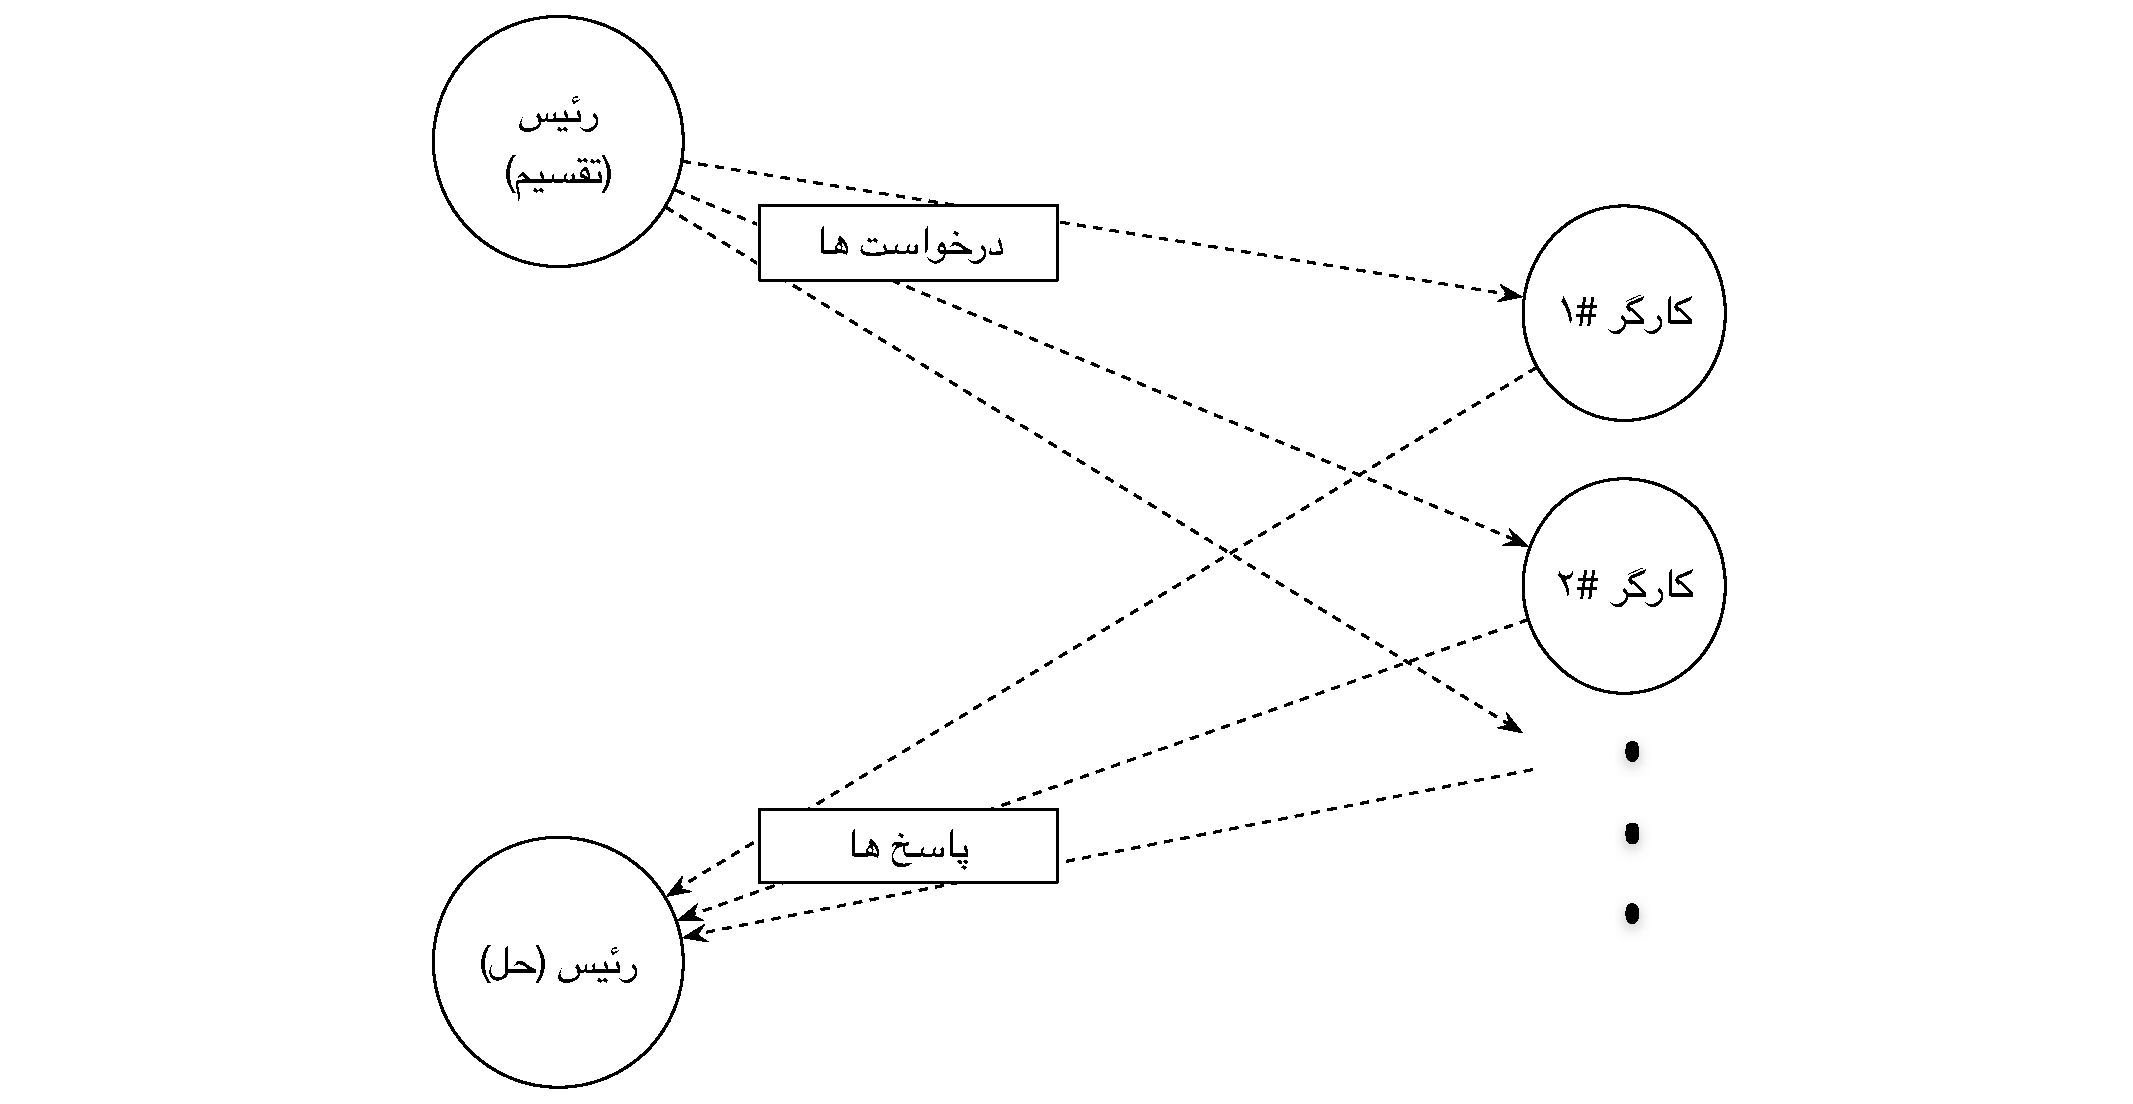
\includegraphics[width=16cm]{3-RelatedWork/Figures/Divide_and_Conquer.pdf}
    \end{center}
    \caption{\label{fig:divide_conquer}  شمای کلی از الگوی تقسیم-و-حل در مدل اکتور }
\end{figure*}
شکل \ref{fig:divide_conquer} شمایی از نحوه‌ی پیاده‌سازی الگوی تقسیم-و-حل در مدل اکتور را نمایش می‌دهد.\\
الگوی خط لوله برای حالت‌هایی مناسب است که فعالیت قابل تقسیم به بخش‌های افزایشی باشد. در این صورت هر اکتور تغییرات مربوطه را در مدل ایجاد می‌کند و آن را به عنوان پیغام به اکتور بعدی در خط لوله منتقل می‌کند.

\begin{figure*}
    \begin{center}
	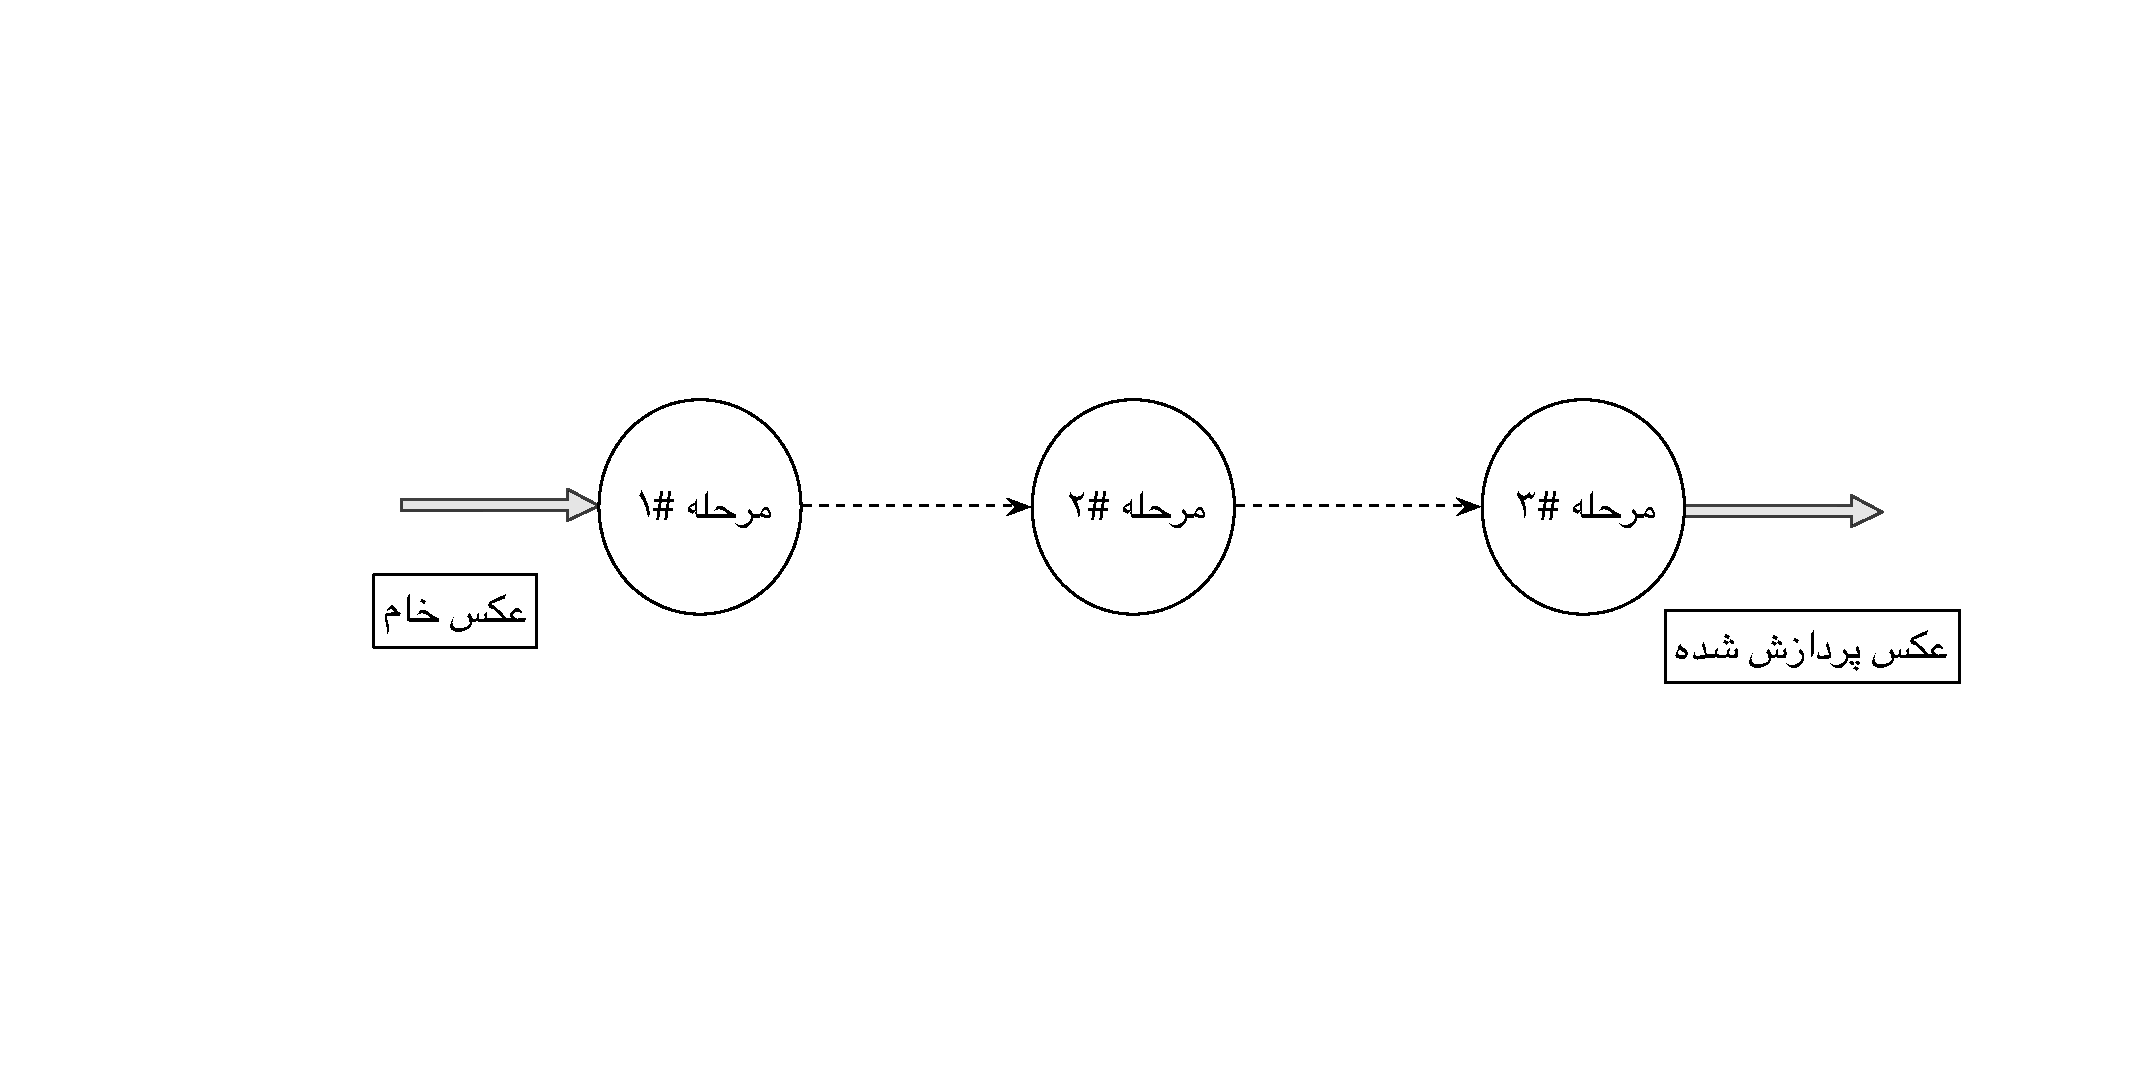
\includegraphics[width=16cm]{3-RelatedWork/Figures/pipeline.pdf}
    \end{center}
    \caption{\label{fig:pipeline}  مثالی از الگوی خط لوله (پردازش تصویر) }
\end{figure*}
به عنوان مثالی از الگوی خط لوله یک برنامه‌ی پردازش تصویر را در نظر بگیرید. هر مرحله از خط لوله، تغییراتی را در تصویر دریافتی ایجاد می‌کند و تصویر نتیجه را به مرحله‌ی بعد منتقل می‌کند. در پیاده‌سازی با روش اکتور، هر مرحله به صورت یک اکتور مدل می‌شود و تصویر به صورت پیغام بین مراحل رد و بدل می‌شود. در شکل \ref{fig:pipeline} شمایی از این الگو نشان داده شده‌ است. \\
در بررسی‌های انجام شده مشخص شد که در پژوهش‌های مذکور، الگوهای ارائه شده صرفا الگوهای کلی همروندی هستند و اشکال مختلف استفاده از آنها و همچنین تاثیر استفاده از این الگوها در طراحی منطق دامنه در این پژوهش‌ها ارائه نشده است.

\section{ همگام‌سازی و هماهنگی اکتورها }
\label{section:coordinationAndSyncronization}
همان‌طور که در بخش‌های قبل ذکر شد،  مدل اکتور دارای خاصیت ناهمگامی‌ است و ترتیب پیغام‌هایی که یک اکتور دریافت می‌کند وابسته به ترتیب فرستاده شدن پیغام‌ها نیست. نتیجه‌ی این خاصیت این است که تعداد ترتیب\LTRfootnote{ordering}‌های دریافت پیغام‌ها در مدل اکتور نمایی است\cite{KarmaniAgha_Actors_11}. به دلیل اینکه فرستنده‌ی پیغام از حالت محلی اکتور گیرنده اطلاعی ندارد، ممکن است بعضی از ترتیب‌های ذکر شده برای پیغام‌ها مطلوب نباشد. به عنوان مثال الگوریتمی را در نظر بگیرید که زیر بخش‌های مختلف آن به اکتور‌هایی فرستاده شده و نتایج آن دریافت می‌شود ولی در آن ترتیب دریافت نتایج اهمیت داشته باشد.  نیاز به این نوع اولویت‌بندی‌ها در مدل اکتور منجر به ایجاد پیچیدگی در محاسبات همروند می‌شود و در صورت پیاده‌سازی نامناسب باعث ایجاد ناکارامدی در برنامه‌ها می‌شود. راه حل این مسئله در مدل اکتور همگام‌سازی است. در مدل اکتور، اکتور‌ها برای همگام‌سازی باهم ارتباط برقرار می‌کنند. در این قسمت دو نوع الگوی هماهنگی اکتور‌ها را معرفی می‌کنیم: تبادل پیغام شبه آرپی‌سی (فراخوانی رویه راه دور)\LTRfootnote{Remote Procedure Call} و قیود همگام‌سازی محلی \LTRfootnote{Local Synchronization Constraints}. \cite{Agha1990,Agha93abstractionand,Papaioannou,KarmaniAgha_Actors_11} 
\subsection{تبادل پیغام شبه-آرپی‌سی}
در ارتباط شبه‌-آرپی‌سی، فرستنده‌ پس از ارسال پیغام منتظر گرفتن پیغام پاسخ از طرف گیرنده می‌ماند. رفتار اکتور در این مدل به ترتیب زیر است:
\begin{enumerate}
\item اکتور فرستنده درخواست را در قالب یک پیغام به اکتور گیرنده ارسال می‌کند.
\item سپس فرستنده صندوق پیغام‌ها را بررسی می‌کند.   
\item اگر پیغام بعدی پاسخ درخواست ارسال شده باشد اقدام مناسب صورت می‌گیرد و فعالیت اکتور ادامه پیدا می‌کند.
\item اگر پیغام بعدی پاسخ درخواست ارسال شده نباشد پیغام جاری در صورت امکان (بسته به منطق برنامه) پردازش می‌شود و در غیر این صورت برای پردازش در آینده به صندوق پیغام‌ها برگردانده می‌شود.
\end{enumerate}
شکل \ref{fig:rpc} مثالی از  پیاده‌سازی ارتباط شبه-آرپی‌سی در مدل اکتور را نشان می‌دهد. ارتباط شبه-آرسی‌پی در دو نوع سناریوی خاص مفید و ضروری است: یک سناریو این است که اکتور نیاز به ارسال پیغام به صورت ترتیبی به یک یا چند اکتور خاص دارد و تا حاصل شدن اطمینان از رسیدن پیغام قبلی پیغام بعد را ارسال نمی‌کند. سناریوی دوم این است که حالت\LTRfootnote{state} اکتور فرستنده بستگی به محتوای پاسخ دارد. در این حالت اکتور قبل از دریافت پاسخ مورد نظر، نمی‌تواند پیغام‌های بعدی را به درستی پردازش کند. نکته‌ی قابل توجه این است که با توجه به شباهت ارسال پیغام شبه-آرپی‌سی به فراخوانی رویه\LTRfootnote{procedure}‌ها در زبان‌های \gls{ترتیبی}\LTRfootnote{sequential}، معمولا برنامه‌نویسان گرایش به استفاده‌ی بیش از حد از این نوع تبادل پیغام دارند که این ممکن است با ایجاد وابستگی‌های بی‌مورد در اشیاء برنامه، علاوه بر کاهش کارایی، منجر به ایجاد \gls{بن‌باز}\LTRfootnote{live lock} در برنامه شود (حالتی که یک اکتور به علت انتظار برای پاسخی که هرگز دریافت نخواهد کرد، از پیغام‌های جدید مرتباً چشم‌پوشی می‌کند یا پردازش آنها را به تأخیر می‌اندازد).\\
امکان تبادل پیغام شبه-آرپی‌سی تقریبا در تمامی پیاده‌سازی‌های مدل اکتور به صورت امکانات سطح زبان وجود دارد\cite{ActorsJVM2009}.

\begin{figure*}
    \begin{center}
	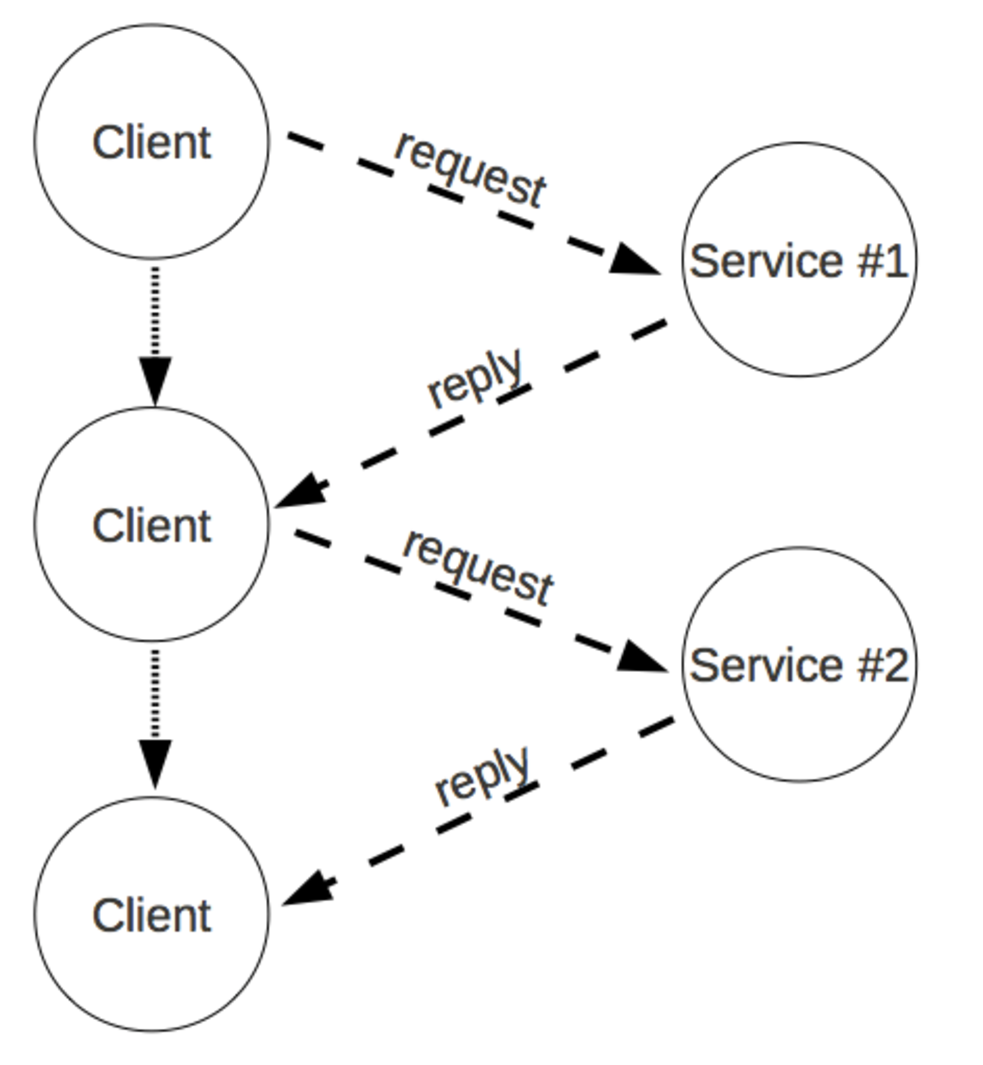
\includegraphics[width=10cm]{3-RelatedWork/Figures/RPC.pdf}
    \end{center}
    \caption{\label{fig:rpc} مثالی از ارتباط شبه-آرپی‌سی در اکتورها) }
\end{figure*}

\subsection{قیود همگام‌سازی محلی}
\label{subsec:local_sync_constraints}
استفاده از قیود همگام‌سازی محلی روشی برای اولیت‌بندی پردازش پیغام‌ها در مدل اکتور است\cite{FrolundCoord}. برای توضیح مفهوم همگام‌سازی محلی مثالی در شکل \ref{fig:lsc} ارائه شده است. در این مثال اکتور فایل پس از دریافت پیغام باز کردن فایل\LTRfootnote{open}، با استفاده از قیود همگام‌سازی خود را محدود به پردازش پیغام‌های \textit{بستن} , \textit{خواندن} می‌کند. در صورت عدم وجود امکانات مناسب برای قیود همگام‌سازی، برنامه‌نویس ناگزیر خواهد بود تا در میان منطق اجرای پیغام‌ها، میانگیر صندوق پیغام‌ها را بررسی و ترکیب یا ترتیب آنها را تغییر داده و یا با جستجو در آنها پیغام مناسب را انتخاب کند. این امر موجب مخلوط شدن منطق چگونگی پردازش پیغام  (چگونه) با منطق زمانی انتخاب پیغام (چه زمانی) می‌شود که در اصول نرم‌افزار پدیده‌ی نامطلوبی به حساب می‌آید\cite{KarmaniAgha_Actors_11}. به همین دلیل بسیاری از زبان‌ها و چارچوب‌های مبتنی بر اکتور امکانات مناسبی برای پشتیبانی از قیود‌ همگام‌سازی محلی ارائه داده‌اند. به عنوان مثال در کتابخانه‌ی اکتور اسکالا که در بخش \ref{section:scalaActorLib} معرفی شد، از مکانیزم تطابق الگو\LTRfootnote{pattern matching} برای اولیت بندی پردازش پیغام‌ها بدون اینکه با منطق اجرایی برنامه مخلوط گردد استفاده می‌شود.



\begin{figure*}
    \begin{center}
	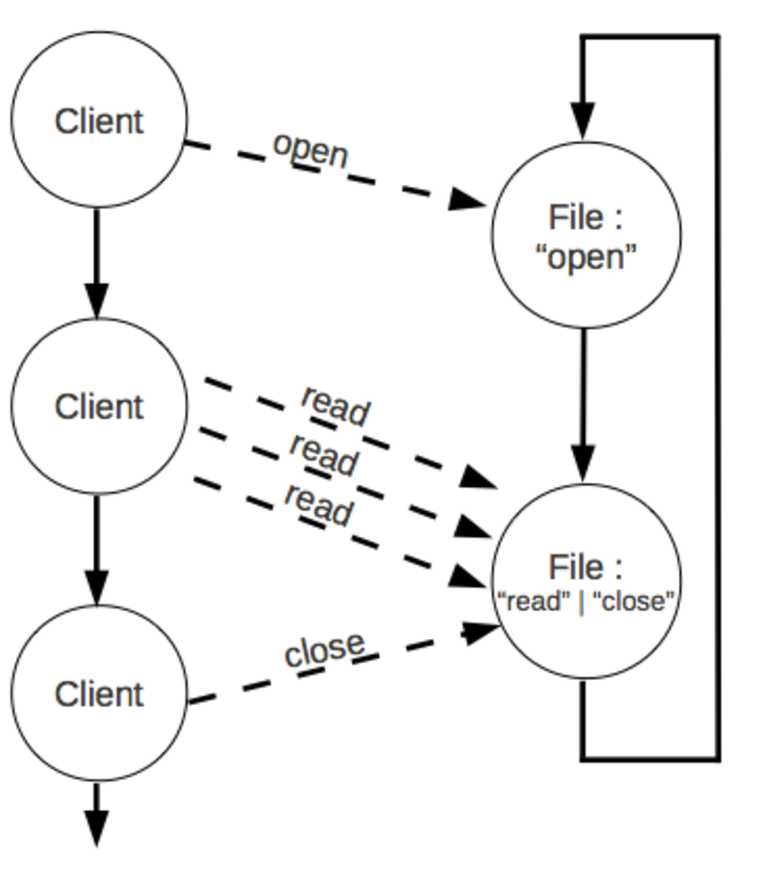
\includegraphics[width=10cm]{3-RelatedWork/Figures/LSC.pdf}
    \end{center}
    \caption{\label{fig:lsc} مثالی از قیود همگام‌سازی محلی. اکتور فایل به وسیله‌ی قیود همگام‌سازی محدود شده است. فلش عمودی به معنی ترتیب زمانی و برچسب‌های داخل دایره به معنی پیغام‌های قابل پردازش در هر حالت هستند. ) }
\end{figure*}
 بررسی پژوهش‌های یاد شده نشان می‌دهد که این پژوهش‌ها تاثیر متقابل منطق دامنه از یک سو و روش‌های هماهنگی و همگام‌سازی در اکتورها از سوی دیگر را بررسی نکرده‌اند. علاوه بر این، در بسیاری از موارد (مانند قیود همگام‌سازی محلی) حوزه‌ی پژوهش بیشتر مربوط به امکانات زبان‌های برنامه‌نویسی همروند مبتنی بر اکتور است و تأثیر این امکانات بر طراحی سیستم بررسی نشده است.
